\section{Simulation Rules} \label{rules}

The simulation runs in discrete steps (\textbf{turns}). The conceptual ``length'' of a turn is
designed to simulate the time to send $k$ bytes, where $k$ is a configurable constant. Each turn, an agent may do any combination of the following: listen, broadcast, move, or die.

\subsection{Movement}

The simulation world consists of a $w$*$h$ grid of signed integers. If a cell's value $c$ is
non-negative, it is the terrain height. Otherwise, the cell is impassable. An agent can move at most
one cell up, down, left, or right per turn. However, after moving into a square, it must wait $c$
turns before it may make another move.

An agent's move may succeed or fail. If an agent tries to move into an impassible cell, it will
fail. It will also fail if it tries to move into a cell that was occupied by another agent at the
end of the last turn, \textbf{or} a cell that another agent attemps to move into in the same turn.
These cases are shown in figure \ref{mvt}.

\begin{figure*}[h!]
    \begin{center}
        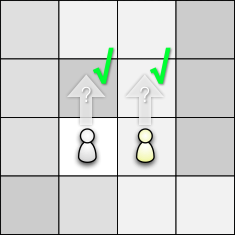
\includegraphics[width=1in]{figures/mvt1.png}
        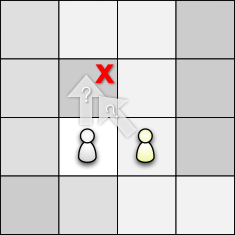
\includegraphics[width=1in]{figures/mvt2.png}
        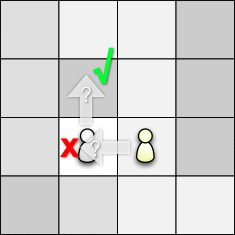
\includegraphics[width=1in]{figures/mvt3.png}
    \end{center}
    \caption{Three main cases for movement.}
    \label{mvt}
\end{figure*}

It may seem more intuitive for both moves in case 3 to succeed, i.e. a move $Z\rightarrow Y$ should
succeed if agent $A$ moves $X\rightarrow Y$. However, allowing this case would introduce large
dependency graphs that would span a large geographical area. This kind of dependency graph would
greatly reduce the effectiveness of our horizontal scaling scheme based on geographical partitioning
described later in this paper.

\subsection{Messages}

The broadcast messages agents can send are a simpilification of radio communication. There are $N$
frequencies an agent can broadcast on or listen too. An agent may broadcast a message of 1024 bytes
on a single frequency. The agent may also listen for messages on $M$ frequencies each turn where $M
\leq N$.

Like radio communication, the messages broadcast decay over distance. When an agent listens to a
frequency, the agent always recieves data. However, if no one is broadcasting on that frequency, the
agent will recieve random data. Since the message decays over distance, even if an agent hears it
some parts of the message may be corrupted. The farther away a listener is from a sender, the more
corruption is in the message.

Finally, if more than one message can be heard from the same position, the messages will be combined
probabilistically.

% Finally, if messages cross each other the following algorithm will be used to resolve the
% conflict. First, for each message the message will be corrupted based on its distance to its source,
% just as in the single broadcaster senario. Then, for each bit in each message their will be a
% probability K that the bit will be heard. The probablity will also be based on the distance to the
% source of the message. All of the bits that are heard are XORed together creating a composite
% message. If not bit are heard for a particular bit location a random value is chosen for that bit.

\subsection{Perception}

Agents may or may not be informed of their global position in the world. They also have some way of
``seeing'' nearby agents.

\subsection{Food}

Agents must search the grid to find food. If their coordinator calculates that their food counter is
below zero, they disappear from the grid.

\section{Usefulness of the Simulation}

The simulation provides a close enough approximation of the real world to allow testing of
high-level coordination algorithms to be tested using a very simple API.

The rules for movement (1 delayed turn per cell height difference) and perception provide an
opportunity to experiment with pathfinding algorithms in an environment where little information
outside a limited area is available, similar to the conditions of the DARPA autonomous vehicle
events.

The rules for communication force agents to communicate with distant agents by passing messages
through nearby agents, creating ad-hoc wireless networks. Our messaging system is meant to model the
difficulties of real world radio communication. This will make our simulation a useful tool for
simulating adhoc wireless networks allowing protocol research to be conducted without hardware.
